\documentclass[14pt,a4paper,russian]{extreport}
%===========================================
\usepackage{geometry} 
\usepackage{enumitem}
\usepackage{graphicx}
\usepackage[russian,english]{babel}
\usepackage[T2A]{fontenc}
\usepackage[utf8]{inputenc}
\usepackage{titlesec}
\usepackage{indentfirst}
\usepackage[hidelinks]{hyperref}
%===========================================

%===========================================
\setlength{\parindent}{1.25cm}
\linespread{1.5}

\geometry{
    a4paper,
    total={170mm,257mm},
    top=20mm,
    right=15mm,
    left=25mm
}

\hypersetup{
    citecolor=black,
    filecolor=black,
    linktoc=all,
}

\titleformat{\chapter}{\normalfont\Large\bfseries\filcenter}{Глава \thechapter}{1em}{}
\titleformat{\section}{\normalfont\large\bfseries\filcenter}{\thesection}{1em}{}
\titleformat{\subsection}{\normalfont\bfseries\filcenter}{\thesubsection}{1em}{}

\graphicspath{ {./images/} }
\setlist[enumerate]{label*=\arabic*.}

\bibliographystyle{gost71u} 
%===========================================


\begin{document}

%==============START TITLEPAGE=============
\begin{titlepage}
    \centering
    \begin{figure}
        \center
\includegraphics[width=4cm]{stankin.png}
    \end{figure}
    \textbf {МИНОБРНАУКИ РОССИИ}\par
    {\textbf{федеральное государственное бюджетное образовательное \\учреждение
    высшего образования\\
     «Московский государственный технологический университет «СТАНКИН»\\
     (ФГБОУ ВО МГТУ «СТАНКИН»)}}\par
\hrulefill\par
     {\textbf{Институт}}\hfill{\textbf{Кафедра\phantom{-00000000000-0--}}}\\
     информационных систем и технологий\hfillинформационных систем\phantom{---0-}\\
    \vspace{1cm} 
    {\textbf {Отчёт по самостоятельной работе}\par}
    {по дисциплине {\textbf{«Управление данными»}}\par}
    на тему: \textbf{Проектирование базы данных поликлиники}
    \vspace{3cm}
    \begin{flushleft}
        {\textbf{Студент}  \hfill \rule{2cm}{0.4pt}\phantom{00}Махмудов Б.Н.\phantom{-0}}\par
        {группа ИДБ-16-07\hfill
        \small{подпись}\phantom{0000000000000000000000}}\par
        \vspace{1cm}
        {\textbf{Руководитель}\hfill \rule{2cm}{0.4pt}\phantom{00}Быстрикова
        В.А.}\par
        {Старший преподователь\hfill
        \small{подпись}\phantom{0000000000000000000000}}\par
    \end{flushleft} 
    {\vfill Москва 2018}
\end{titlepage}
%==============END TITLEPAGE=============

\addtocounter{page}{1}

\selectlanguage{russian}

\tableofcontents{}

\newpage

\sloppy

\chapter{Анализ предметной области}

\section{Определение анализа предметной области}

\subsection{Предметная область}
Предметная область — множество всех предметов, свойства которых и отношения между которыми
рассматриваются в научной теории. В логике — подразумеваемая область возможных значений предметных
переменных логического языка.

Предметная область — часть реального мира, рассматриваемая в пределах данного контекста. Под
контекстом здесь может пониматься, например, область исследования или область, которая является
объектом некоторой деятельности.\cite{domainknowladge}

\subsection{Информационный анализ предметной области}
Деятельность, направленная на выявление реальных потребностей заказчика, а также на выяснения
смысла высказанных требований, называется анализом предметной области.
Одна из первых задач, с решением которых сталкивается разработчик программной системы - это
изучение, осмысление и анализ предметной области. Дело в том, что предметная область сильно влияет
на все аспекты проекта: требования к системе, взаимодействие с пользователем, модель хранения
данных, реализацию и т.д.  Анализ предметной области, позволяет выделить ее сущности, определить
первоначальные требования к функциональности и определить границы проекта.


\section{Поликлиника: описание предметной области}
Поликлиника — многопрофильное или специализированное лечебно-профилактическое учреждение для
оказания амбулаторной медицинской помощи больным на приёме и на дому.  На территории России
распределены по территориальному признаку, и являются базовым уровнем медицинского обслуживания
населения.  По мощности городские поликлиники делятся на 5 групп. В структуре городской поликлиники
предусматриваются следующие подразделения:

\begin{enumerate}[noitemsep]
    \item руководство поликлиникой;
    \item регистратура;
    \item кабинет доврачебного приема;
    \item отделение профилактики;
    \item лечебно-профилактические подразделения:
    \item терапевтические отделения;
    \item отделение восстановительного лечения;
    \item отделения по оказанию специализированных видов медицинской помощи (хирургическое,
        гинекологическое) с кабинетами соответствующих специалистов (кардиологический,
        ревматологический, неврологический, урологический, офтальмологический,
        оториноларингологический);
    \item параклинические службы (физиотерапевтический и рентгеновский кабинеты, лаборатории, кабинет
        функциональной диагностики, УЗИ-кабинет);
    \item дневной стационар и стационар на дому;
    \item административно-хозяйственная часть;
    \item врачебные и фельдшерские здравпункты на прикрепленных предприятиях.
\end{enumerate}

Число отделений и кабинетов, их потенциальные возможности определяются мощностью поликлиники и
количеством штатных должностей, которые зависят от численности закрепленного за
поликлиникой населения. Структура поликлиники (открытие тех или иных отделений, кабинетов и
т. п.) зависит от обращаемости населения в это учреждение, от способности поликлиники предоставить
больным необходимую медицинскую помощь.\cite{medstat}

На сегодняшний день автоматизации подвержено подавляющее большинство сфер деятельности человека,
включая здравохранение. Автоматизация здравохранения особенно актуальна ввиду роста человеческого населения
и бюрократизации в сфере оказания медицинских услуг, что приводит к неудобствам и
затруднениям для больных
в получении вышеупомянутых услуг. Но если разработать информационную систему с
централизованной базой данных, позволяющую пользователям удалённо получать справки и записываться
на приём к
врачам, то можно уменьшить нагруженность самого учреждения и улучшить качество услуг для
пациентов. Таким образом автоматизация функционирования
поликлиники, в частности разработка базы данных для неё позволит пациентам сэкономить время на
очередях и бюрократических формальностях, а сотрудникам сосредоточиться непосредственно на
оказании медицинских услуг.


\newpage
\section{Существующие продукты решающие проблему автоматизации}

\subsection{1С : Медицина. Поликлиника}
Прикладное решение «1С:Медицина. Поликлиника» предназначено для автоматизации основных процессов
медицинских организаций различных организационно-правовых форм, оказывающих медицинскую помощь в
амбулаторно-поликлинических условиях. 

\textbf{Функциональные возможности.} 
Прикладное решение «1С:Медицина. Поликлиника» позволяет создать единое информационное пространство
медицинской организации с разделением доступа к данным по ролевому принципу. Имеется возможность
вести учет по нескольким медицинским организациям в одной информационной базе.

Программа позволяет вести несколько медицинских карт для одного пациента - амбулаторную карту,
стоматологическую карту и т.д., пример карты пациента приведён ниже (Рис. \ref{fig:pc}). Для каждого медицинского работника указывается, к какому типу карт
он имеет доступ. В программе имеются гибкие механизмы квотирования, которые позволяют устанавливать
ограничения на объемы оказываемой медицинской помощи. Учет деятельности медицинского персонала
ведется по медицинским услугам. Пример пользвательского интерфейса программы показан на
Рис. \ref{fig:1c}
\begin{figure}[t!]
        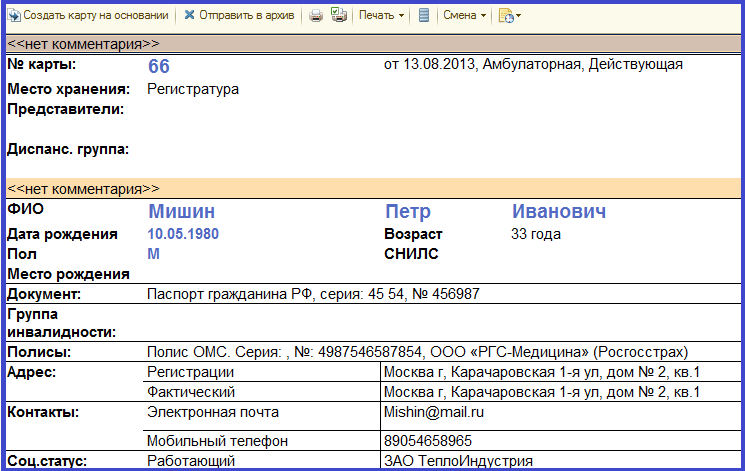
\includegraphics[width=\textwidth]{patientcard}
        \caption{Пример карты пациента}
        \label{fig:pc}
\end{figure}
\par
\begin{figure}[h!]
        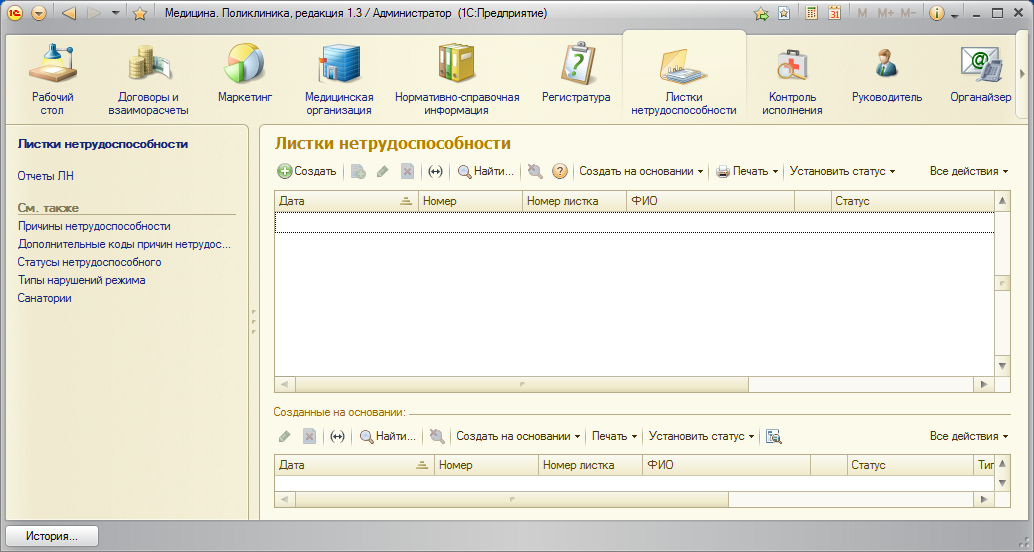
\includegraphics[width=\textwidth]{1cinterface}
        \caption{Пользовательский интерфейс «1С:Медицина. Поликлиника»}
        \label{fig:1c}
\end{figure}

Предварительную запись пациентов может осуществлять как регистратура, так и врачи при выполнении
назначений повторных приемов, консультаций, исследований, манипуляций. Для осуществления
оперативного планирования врачебному медицинскому персоналу и кабинетам задаются графики работы,
нормы загрузки, перечень выполняемых услуг. Оперативное планирование деятельности кабинетов
осуществляется по данным предварительной записи пациентов.\cite{1cclinic}
\cleardoublepage
\begin{figure}[b!]
        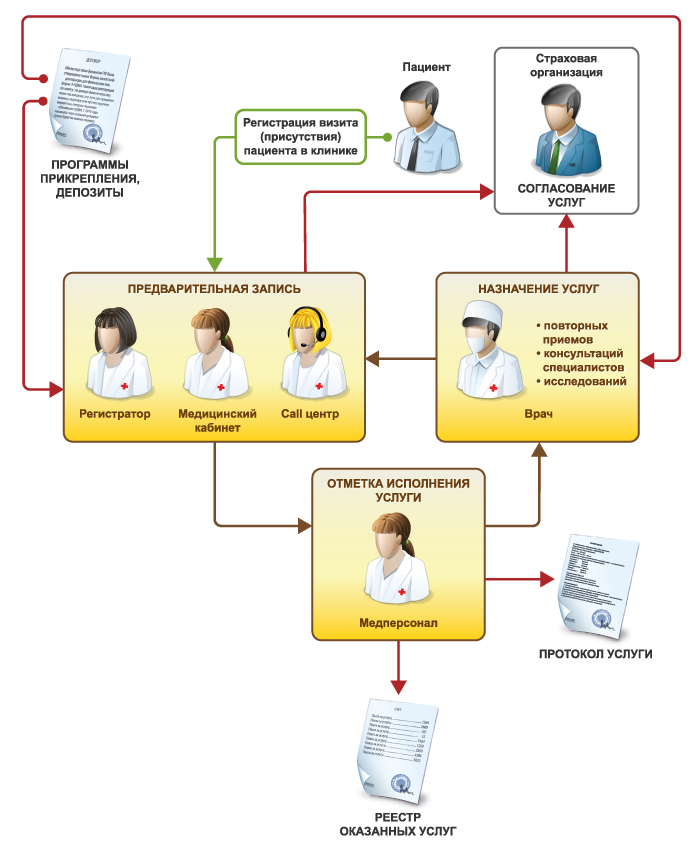
\includegraphics[scale=0.9]{1cdiagram}
        \caption{Диаграмма функционирования «1С:Медицина. Поликлиника»}
        \label{fig:1cdiag}
\end{figure}

В целом процесс работы программного продукта «1С:Медицина. Поликлиника» можно описать с помощью
диаграммы (Рис. \ref{fig:1cdiag}).
\subsection{Сайт частных поликлиник «СМ-Клиника»}
Многопрофильный медицинский холдинг «СМ-Клиника»  - это сеть многопрофильных
медицинских центров для взрослых и детей, основанной в 2002 году.
Сайт компании доступен по адресу \url{http://www.smclinic.ru/}.
Скриншот сайта приведён на Рис. \ref{fig:cc}.\par

\begin{figure}[h!]
        
\includegraphics[width=\textwidth]{cmclinic}
        \caption{Внешний вид сайта «СМ-Клиника»}
        \label{fig:cc}
\end{figure}

\noindent Интерес здесь представляют функции «Записаться на приём» и «Личный кабинет». \par
1-ое позволяет предварительно записаться на приём к лечащему врачу посредством заполнения
со стороны пользователя соответствующей формы (Рис. \ref{fig:appdoc}). Очевидно после отправки
заполненной формы в базе данных поликлиники должна появиться запись о предстоящем визите
пациента.

\begin{figure}[t!]
        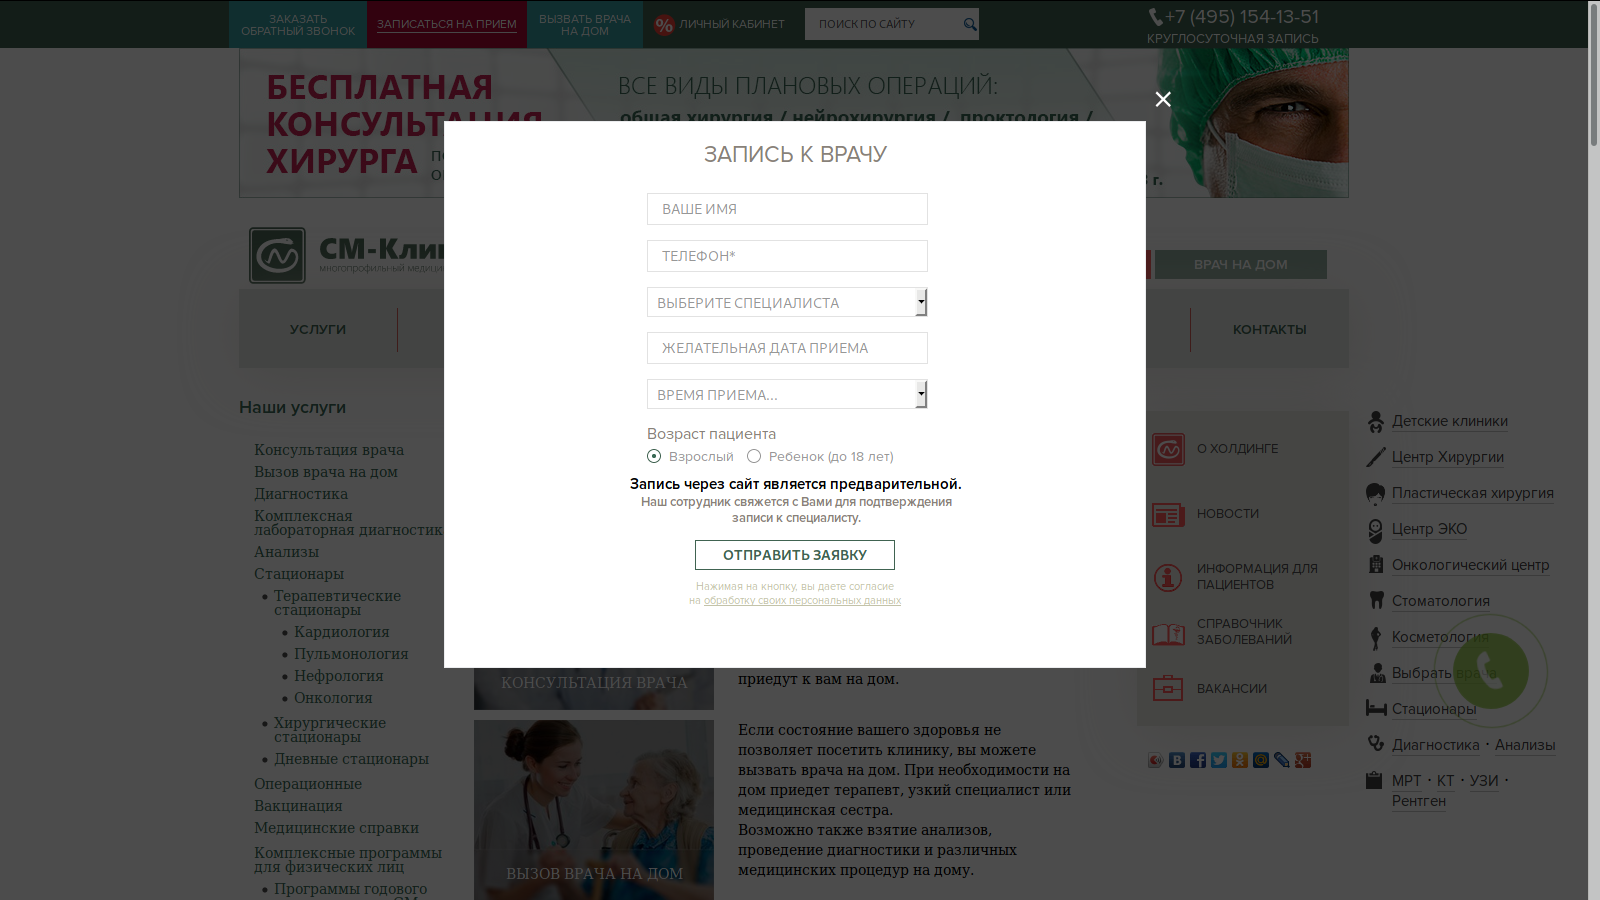
\includegraphics[width=\textwidth]{appdoc}
        \caption{Форма записи на приём к врачу в «СМ-Клиника»}
        \label{fig:appdoc}
\end{figure}

\begin{figure}[b!]
        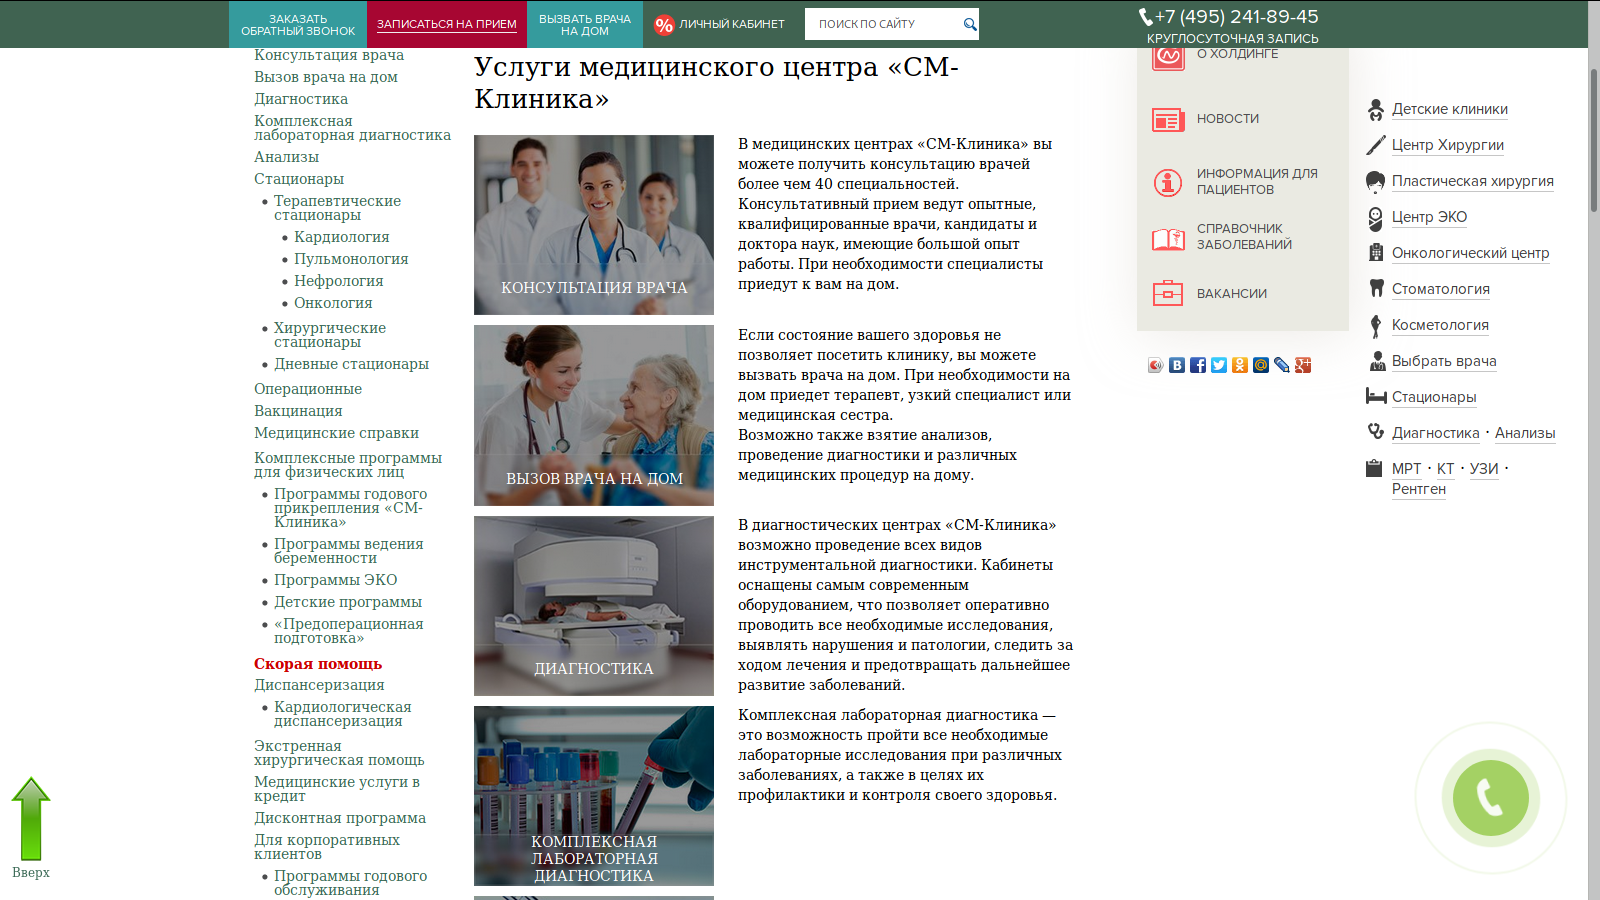
\includegraphics[width=\textwidth]{lkcm}
        \caption{Форма входа в личный кабинет пользователя}
        \label{fig:lkcm}
\end{figure}

\cleardoublepage
Функция «Личный кабинет» (Рис. \ref{fig:lkcm}) предоставляет широкий перечень возможностей для зарегистрированных
пользователей:\cite{smclin}

\begin{enumerate}[noitemsep]
    \item получить доступ к своей медицинской карте - увидеть детальную историю всех посещений
        клиники, фамилии лечащих докторов, их специализации, точные даты посещений и другую
        полезную информацию;

    \item посмотреть назначенную схему лечения, рекомендации лечащих врачей, назначенные
        обследования и др.;

    \item ознакомиться с результатами анализов и обследований, сохранить их на локальный компьютер или
        сразу распечатать;

    \item увидеть, когда лечащий врач пациента работает и какое время для приема на текущий момент у него
        свободно;

    \item самостоятельно записаться к врачу в удобное для пользователя время;

    \item посмотреть текущую скидку пользователя, актуальные акции и предложения клиник;

    \item оставить отзыв о враче или клинике.
\end{enumerate}

\subsection{Сравнение «1С:Медицина. Поликлиника» и сайта поликлиники «СМ-Клиника»}
Прямое сравнение данных продуктов не представляется возможным, так как они ориентированы на две
совершенно разные группы пользователей, сотрудников поликлиники и пациентов соответственно. Как
результат оба продукта обладают не поддающимся непосредственному сравнению возможностями. Данный факт
наталкивает на идею создания информационной экосистемы где вышеупомянутые группы пользователей
имели бы возможность взаимодействовать на базе одной единой платформы. Таким образом описание
системы совмещающей в себе функции двух программных продуктов, которые были рассмотрены в
предыдущих подразделах, и является темой следующего раздела данной курсовой работы.


\section{Фунцкии, планируемые для реализации в курсовом проекте}
Как говорилось раньше, в рамках данной курсовой работы планируется создание единой платформы для
взамодейстивия пациентов с сотрудниками поликлиники. Отсюда вытекает что по сути существует две
различные категории потенциальных пользователей системы, а т.к. и потребности этих категорий вообще
говоря различны, то и при проектировании возможностей системы логично будет придерживаться данного
разделения. Основные функции для реализации, таким образом можно подразделить на 2 группы: 
\begin{enumerate}[noitemsep]
    \item Функции для пациентов:
        \begin{enumerate}[noitemsep]
            \item запись на приём к врачу;
            \item просмотр личных медицинских карт;
            \item просмотр результатов анализов;
            \item ознакомиться с графиком работы врачей.
            \item прамая связь с лечащим врачом;
        \end{enumerate}
    \item Функции для сотрудников:
        \begin{enumerate}
            \item просмотр и/или редактировании медицинских карт;
            \item просмотр и/или редактировании результатов анализов;
            \item запись на приём к врачу;
            \item проcмотр и/или редактирование записей к врачам;
            \item связь с пациентами и другим персоналом;
            \item регистрация нового пользователя;
            \item доступ к личному календарю.
        \end{enumerate}
\end{enumerate}


\chapter{Концептуальное проектирование}
\section{Определение концептуального проектирования}
Концептуальное проектирование технических систем — начальная стадия проектирования, на которой
принимаются решения определяющие последующий облик, и проводится исследование и согласование
параметров созданных технических решений с возможной их организацией. Термин «концепция»
применяется для описания принципа действия не только в технических системах, но и в научных,
художественных и прочих видах деятельности. «Концепт» (лат.) — содержание понятия, смысл. Таким
образом, проектирование на концептуальном уровне — на уровне смысла или содержания понятия систем.
В частности концептуальное (инфологическое) проектирование базы данных — построение семантической модели
предметной области, то есть информационной модели наиболее высокого уровня абстракции. Такая модель
создаётся без ориентации на какую-либо конкретную СУБД и модель данных. Термины «семантическая
модель», «концептуальная модель» и «инфологическая модель» являются синонимами. Кроме того,
в этом контексте равноправно могут использоваться слова «модель базы данных» и «модель
предметной области» (например, «концептуальная модель базы данных» и «концептуальная модель
предметной области»), поскольку такая модель является как образом реальности, так и
образом проектируемой базы данных для этой реальности.Конкретный вид и содержание концептуальной
модели базы данных определяется выбранным для этого формальным аппаратом. Обычно используются
графические нотации, подобные ER-диаграммам.

ER-модель (от англ. entity-relationship model, модель «сущность — связь») — модель данных,
позволяющая описывать концептуальные схемы предметной области.  ER-модель используется при
высокоуровневом (концептуальном) проектировании баз данных. С её помощью можно выделить ключевые
сущности и обозначить связи, которые могут устанавливаться между этими сущностями.  Во время
проектирования баз данных происходит преобразование ER-модели в конкретную схему базы
данных на основе выбранной модели данных (реляционной, объектной, сетевой или др.). \cite{concept}


\section{Концептуальная модель базы данных поликлиники}
В ходе выполнения анализа предметной области можно выделить следующие задачи, подлежащие решению
для имплементации информационной системы описанной в предыдущей главе.
\begin{enumerate}[noitemsep]
    \item создание единой базы данных (БД) для всех пользователей ИС;
    \item разграничение доступа к БД как между отдельными группами пользователей так и внутри самих групп;
    \item реализация механизма поиска необходимой информации по БД;
    \item реализации методов предоставления соответствующих функций в зависимости от роли и прав
        пользователя;
    \item разработка подсистемы связи между пользователеми с хранением истории непосредственно в
        самой базе данных.
\end{enumerate}
Если же рассматривать данныю ИС с точки зрения возможных вариантов использования, то можно выделить
два действующих лица, сотрудник и пациент. Такое небольшое количество действующих лиц объясняется
тем, что функции, которые будет предоставлять система, подразделены на две основные категории, в то
время как возможности пользователей внутри своей группы будут разграничены при помощи вышестоящего
логического уровня рассматриваемой ИС.



\chapter{Логическое проектирование}

\section{ОСНОВЫ}



\chapter{Физическое проектирование}

\section{SQL}



\bibliography{b}{}
\end{document}

